\subsection{Resultados en los 30 polígonos}
\label{sec:resultados}

Ambos niveles se resolvieron para los 30 polígonos (183.01~ha) con los parámetros de la \cref{sec:validacion}, el mosaico de $4\times13=52$ posiciones y la matriz de la \cref{tab:matriz-competencia}. Todos los resultados se reproducen con \texttt{refor} y la semilla 42.

\subsubsection{Compra}
\label{subsec:res-compra}

\paragraph{El presupuesto no alcanza} Con $B=\$12{,}500$/ha ningún polígono es factible. El presupuesto mínimo es, en promedio ponderado por superficie, $\bar{B}^{*}=\$14{,}496$/ha, 16\,\% más que el disponible: va de \$14{,}361/ha en el polígono 8 a \$14{,}934/ha en el polígono 1. Cumplir la meta en los 30 polígonos con $\alpha=0.05$ requiere \$365~mil adicionales. La infactibilidad es estructural, como anticipaba la estimación de la \cref{subsec:compra-formulacion}: el costo de cubrir el faltante corregido por mortalidad ya excedía el presupuesto antes de agregar margen de seguridad y logística. Aceptar más riesgo apenas ayuda (\cref{tab:frontera}): pasar de $\alpha=0.01$ a $\alpha=0.50$ ahorra 3.7\,\% del presupuesto a cambio de multiplicar por cincuenta la probabilidad de incumplir la meta de cada especie, y aun con $\alpha=0.50$ faltan \$296~mil. Lo que excede el presupuesto es el faltante mismo, no el margen de seguridad. El sobrecosto logístico pesa más que el riesgo: con $\theta=0.10$ en lugar de $0.05$, $\bar{B}^{*}$ sube a \$15{,}186/ha.

\begin{table}[t]
\centering
\caption{Presupuesto mínimo ponderado por superficie, $\bar{B}^{*}$ (\$/ha), con Monte Carlo y con la cola binomial exacta, y faltante respecto a \$12{,}500/ha en los 183.01~ha.}
\label{tab:frontera}
\small
\begin{tabular}{@{}rrrr@{}}
\toprule
$\alpha$ & Monte Carlo & Exacto & Faltante (miles de \$) \\
\midrule
0.01 & 14{,}664 & 14{,}666 & 396 \\
0.02 & 14{,}596 & 14{,}597 & 384 \\
0.05 & \textbf{14{,}496} & \textbf{14{,}496} & \textbf{365} \\
0.10 & 14{,}408 & 14{,}409 & 349 \\
0.20 & 14{,}305 & 14{,}305 & 330 \\
0.30 & 14{,}233 & 14{,}233 & 317 \\
0.50 & 14{,}117 & 14{,}118 & 296 \\
\bottomrule
\end{tabular}
\end{table}

\paragraph{Compra sin presupuesto} Sin la restricción \eqref{eq:presupuesto}, la compra óptima suma $108{,}680$ plantas y \$2.65~millones, 593.8 plantas/ha. Con las 128.8 plantas/ha existentes, la densidad al plantar es de 722.6 plantas/ha, 9.8\,\% sobre la meta: es la sobreplantación que absorbe la mortalidad del primer año con la confiabilidad exigida. El costo esperado de reposición es de apenas \$5/ha, porque con $\alpha=0.05$ el déficit esperado es casi nulo y el costo es casi todo de adquisición.

\paragraph{Composición} La composición óptima agota la banda \eqref{eq:banda} en la dirección que anticipaba el costo por planta sobreviviente $c_s/q_s$ (\cref{tab:compra-parametros}). Las cuatro especies de \textit{Opuntia}, las de menor $c_s/q_s$, suben entre 9.4\,\% y 9.9\,\% respecto al plan; \textit{P.~laevigata}, \textit{A.~scabra} y \textit{Y.~filifera}, las de mayor, bajan entre 9.2\,\% y 9.9\,\%; \textit{A.~lechuguilla} y \textit{A.~striata} bajan 8\,\%, y \textit{A.~salmiana} se mantiene. El margen de ajuste por especie, que el plan concibe como tolerancia de campo, resulta ser la principal palanca de costo del modelo.

\paragraph{Tamaño del polígono} Los dos polígonos más chicos son los más caros por hectárea (\$14{,}934 en el polígono 1, de 1.28~ha, y \$14{,}819 en el 4, de 1.38~ha), y la correlación entre superficie y $B_i^{*}$ es de $-0.63$. El margen necesario para cumplir con probabilidad $1-\alpha$ crece aproximadamente con la raíz de la meta, más lento que la meta misma, de modo que pesa más por hectárea cuando la meta es chica. La relación no es estricta porque $B_i^{*}$ también depende de cuántas plantas existentes tiene cada polígono.

\subsubsection{Distribución espacial}
\label{subsec:res-espacial}

\paragraph{Seis claves para 30 polígonos} Al repartir la compra sin presupuesto de cada polígono en 52 posiciones, los 30 polígonos se reducen a seis composiciones distintas y, por tanto, a seis claves de plantación (\cref{tab:res-mosaicos}). La primera la comparten 18 polígonos y la segunda, 5. En la práctica, la cuadrilla necesita solo seis tablas de claves para todo el sitio.

\begin{table}[t]
\centering
\caption{Claves de plantación. $n_p$: polígonos que comparten la clave; azar: competencia esperada de una asignación aleatoria con la misma composición, \cref{eq:competencia-azar}; memético: mejor competencia de 30 corridas; reducción: $1-C/\mathbb{E}[C]$.}
\label{tab:res-mosaicos}
\small
\begin{tabular}{@{}crrrr@{}}
\toprule
Clave & $n_p$ & Azar & Memético & Reducción (\%) \\
\midrule
1 & 18 & 93.34 & 78.18 & 16.2 \\
2 &  5 & 92.37 & 77.37 & 16.2 \\
3 &  1 & 95.09 & 81.29 & 14.5 \\
4 &  1 & 91.74 & 76.77 & 16.3 \\
5 &  4 & 91.73 & 76.80 & 16.3 \\
6 &  1 & 95.90 & 81.85 & 14.6 \\
\bottomrule
\end{tabular}
\end{table}

\paragraph{Reducción de la competencia} El memético reduce la competencia entre 14.5\,\% y 16.3\,\% respecto a una asignación aleatoria de igual composición. Las claves 3 y 6, de un solo polígono cada una, reducen menos porque tienen 6 posiciones de \textit{P.~laevigata} en lugar de 7, es decir, un separador menos, como se explica enseguida.

\paragraph{Estructura de las claves} La \cref{fig:clave1} muestra la clave 1. De los 156 pares de vecinas de cada mosaico, solo uno o dos son de la misma especie, y en todos los casos son de \textit{A.~salmiana}, que ocupa entre 27\,\% y 29\,\% de las posiciones. \textit{P.~laevigata}, con la mayor penalización intraespecífica (1.50), nunca queda junto a otra de su especie y actúa como separador: entre 45\,\% y 50\,\% de sus vecinas son \textit{A.~salmiana} y entre 29\,\% y 39\,\% \textit{O.~streptacantha}, las dos especies abundantes con penalización intraespecífica alta, con las que la suya es mínima (0.20 y 0.17). Es justo el arreglo de nodriza que motivó el término $F_{ab}$ de la matriz: cada mezquite queda rodeado de suculentas.

\paragraph{Comparación con la clave vigente} El orden de plantación que usa CONAFOR es una secuencia de 22 posiciones para cada 100~m lineales, con la composición del plan (siete \textit{A.~salmiana}, tres \textit{P.~laevigata} y entre una y dos de cada especie restante). Al ser una sola fila, la secuencia no dice cómo se acomodan las filas entre sí, y en el tresbolillo cada planta tiene dos vecinas en la fila anterior y dos en la siguiente. Se evaluó la secuencia en la retícula con la matriz $W$ para los 22 desfases posibles entre filas consecutivas (\cref{tab:clave-vigente}). Si cada fila repite la secuencia alineada con la anterior, cada planta queda junto a dos de su misma especie y la competencia es 13\,\% \emph{mayor} que la de una asignación al azar con la misma composición (coeficiente 1.13). Con el mejor desfase, de cinco posiciones, el coeficiente baja a 0.85, y el promedio de los 22 desfases es 0.94. La clave 1 del memético (coeficiente 0.84) mejora a la vigente en cualquier desfase, aunque frente al mejor de ellos la diferencia es pequeña; por par de vecinas, su competencia es 29\,\% menor que la de la secuencia alineada y 6\,\% menor que la del mejor desfase, aunque esta comparación mezcla dos composiciones distintas, la del plan y la de la compra. La mayor ganancia, por tanto, no viene solo de optimizar, sino de especificar el arreglo en dos dimensiones: una tabla de claves fija las vecinas de cada planta en todas las direcciones, mientras que una secuencia por fila deja la mitad de las vecindades al azar del desfase con que se empiece cada fila.

\begin{table}[t]
\centering
\caption{Clave vigente de 22 posiciones evaluada en el tresbolillo según el desfase entre filas consecutivas, frente a la clave 1 del memético. Coeficiente: competencia entre la esperada al azar con la misma composición; por par: competencia media por par de vecinas; mismas: vecinas de la misma especie por planta.}
\label{tab:clave-vigente}
\small
\begin{tabular}{@{}lrrr@{}}
\toprule
Arreglo & Coeficiente & Por par & Mismas \\
\midrule
Vigente, filas alineadas & 1.126 & 0.709 & 2.00 \\
Vigente, mejor desfase (5) & 0.850 & 0.535 & 0.09 \\
Vigente, media de los 22 desfases & 0.944 & 0.594 & 0.64 \\
Memético, clave 1 & 0.838 & 0.501 & 0.08 \\
\bottomrule
\end{tabular}
\end{table}

\begin{figure}
\centering
% Generado por scripts/figura_clave.py; no editar a mano.
% Mosaico 1: competencia 78.18, al azar 93.3365.
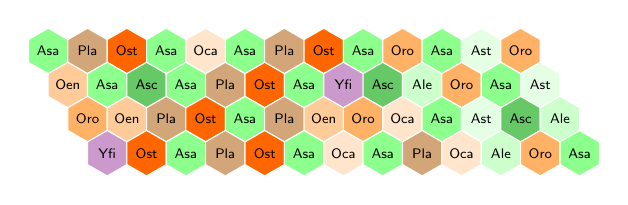
\begin{tikzpicture}[x=0.5cm,y=0.5cm,font=\sffamily\fontsize{4.5}{5}\selectfont]
  \filldraw[fill=green!45,draw=white,line width=0.4pt] (0.000,0.577) -- (-0.500,0.289) -- (-0.500,-0.289) -- (-0.000,-0.577) -- (0.500,-0.289) -- (0.500,0.289) -- cycle;
  \node at (0.000,0.000) {Asa};
  \filldraw[fill=brown!70,draw=white,line width=0.4pt] (1.000,0.577) -- (0.500,0.289) -- (0.500,-0.289) -- (1.000,-0.577) -- (1.500,-0.289) -- (1.500,0.289) -- cycle;
  \node at (1.000,0.000) {Pla};
  \filldraw[fill=orange!80!red,draw=white,line width=0.4pt] (2.000,0.577) -- (1.500,0.289) -- (1.500,-0.289) -- (2.000,-0.577) -- (2.500,-0.289) -- (2.500,0.289) -- cycle;
  \node at (2.000,0.000) {Ost};
  \filldraw[fill=green!45,draw=white,line width=0.4pt] (3.000,0.577) -- (2.500,0.289) -- (2.500,-0.289) -- (3.000,-0.577) -- (3.500,-0.289) -- (3.500,0.289) -- cycle;
  \node at (3.000,0.000) {Asa};
  \filldraw[fill=orange!20,draw=white,line width=0.4pt] (4.000,0.577) -- (3.500,0.289) -- (3.500,-0.289) -- (4.000,-0.577) -- (4.500,-0.289) -- (4.500,0.289) -- cycle;
  \node at (4.000,0.000) {Oca};
  \filldraw[fill=green!45,draw=white,line width=0.4pt] (5.000,0.577) -- (4.500,0.289) -- (4.500,-0.289) -- (5.000,-0.577) -- (5.500,-0.289) -- (5.500,0.289) -- cycle;
  \node at (5.000,0.000) {Asa};
  \filldraw[fill=brown!70,draw=white,line width=0.4pt] (6.000,0.577) -- (5.500,0.289) -- (5.500,-0.289) -- (6.000,-0.577) -- (6.500,-0.289) -- (6.500,0.289) -- cycle;
  \node at (6.000,0.000) {Pla};
  \filldraw[fill=orange!80!red,draw=white,line width=0.4pt] (7.000,0.577) -- (6.500,0.289) -- (6.500,-0.289) -- (7.000,-0.577) -- (7.500,-0.289) -- (7.500,0.289) -- cycle;
  \node at (7.000,0.000) {Ost};
  \filldraw[fill=green!45,draw=white,line width=0.4pt] (8.000,0.577) -- (7.500,0.289) -- (7.500,-0.289) -- (8.000,-0.577) -- (8.500,-0.289) -- (8.500,0.289) -- cycle;
  \node at (8.000,0.000) {Asa};
  \filldraw[fill=orange!60,draw=white,line width=0.4pt] (9.000,0.577) -- (8.500,0.289) -- (8.500,-0.289) -- (9.000,-0.577) -- (9.500,-0.289) -- (9.500,0.289) -- cycle;
  \node at (9.000,0.000) {Oro};
  \filldraw[fill=green!45,draw=white,line width=0.4pt] (10.000,0.577) -- (9.500,0.289) -- (9.500,-0.289) -- (10.000,-0.577) -- (10.500,-0.289) -- (10.500,0.289) -- cycle;
  \node at (10.000,0.000) {Asa};
  \filldraw[fill=green!10,draw=white,line width=0.4pt] (11.000,0.577) -- (10.500,0.289) -- (10.500,-0.289) -- (11.000,-0.577) -- (11.500,-0.289) -- (11.500,0.289) -- cycle;
  \node at (11.000,0.000) {Ast};
  \filldraw[fill=orange!60,draw=white,line width=0.4pt] (12.000,0.577) -- (11.500,0.289) -- (11.500,-0.289) -- (12.000,-0.577) -- (12.500,-0.289) -- (12.500,0.289) -- cycle;
  \node at (12.000,0.000) {Oro};
  \filldraw[fill=orange!40,draw=white,line width=0.4pt] (0.500,-0.289) -- (-0.000,-0.577) -- (0.000,-1.155) -- (0.500,-1.443) -- (1.000,-1.155) -- (1.000,-0.577) -- cycle;
  \node at (0.500,-0.866) {Oen};
  \filldraw[fill=green!45,draw=white,line width=0.4pt] (1.500,-0.289) -- (1.000,-0.577) -- (1.000,-1.155) -- (1.500,-1.443) -- (2.000,-1.155) -- (2.000,-0.577) -- cycle;
  \node at (1.500,-0.866) {Asa};
  \filldraw[fill=green!65!black!60,draw=white,line width=0.4pt] (2.500,-0.289) -- (2.000,-0.577) -- (2.000,-1.155) -- (2.500,-1.443) -- (3.000,-1.155) -- (3.000,-0.577) -- cycle;
  \node at (2.500,-0.866) {Asc};
  \filldraw[fill=green!45,draw=white,line width=0.4pt] (3.500,-0.289) -- (3.000,-0.577) -- (3.000,-1.155) -- (3.500,-1.443) -- (4.000,-1.155) -- (4.000,-0.577) -- cycle;
  \node at (3.500,-0.866) {Asa};
  \filldraw[fill=brown!70,draw=white,line width=0.4pt] (4.500,-0.289) -- (4.000,-0.577) -- (4.000,-1.155) -- (4.500,-1.443) -- (5.000,-1.155) -- (5.000,-0.577) -- cycle;
  \node at (4.500,-0.866) {Pla};
  \filldraw[fill=orange!80!red,draw=white,line width=0.4pt] (5.500,-0.289) -- (5.000,-0.577) -- (5.000,-1.155) -- (5.500,-1.443) -- (6.000,-1.155) -- (6.000,-0.577) -- cycle;
  \node at (5.500,-0.866) {Ost};
  \filldraw[fill=green!45,draw=white,line width=0.4pt] (6.500,-0.289) -- (6.000,-0.577) -- (6.000,-1.155) -- (6.500,-1.443) -- (7.000,-1.155) -- (7.000,-0.577) -- cycle;
  \node at (6.500,-0.866) {Asa};
  \filldraw[fill=violet!40,draw=white,line width=0.4pt] (7.500,-0.289) -- (7.000,-0.577) -- (7.000,-1.155) -- (7.500,-1.443) -- (8.000,-1.155) -- (8.000,-0.577) -- cycle;
  \node at (7.500,-0.866) {Yfi};
  \filldraw[fill=green!65!black!60,draw=white,line width=0.4pt] (8.500,-0.289) -- (8.000,-0.577) -- (8.000,-1.155) -- (8.500,-1.443) -- (9.000,-1.155) -- (9.000,-0.577) -- cycle;
  \node at (8.500,-0.866) {Asc};
  \filldraw[fill=green!20,draw=white,line width=0.4pt] (9.500,-0.289) -- (9.000,-0.577) -- (9.000,-1.155) -- (9.500,-1.443) -- (10.000,-1.155) -- (10.000,-0.577) -- cycle;
  \node at (9.500,-0.866) {Ale};
  \filldraw[fill=orange!60,draw=white,line width=0.4pt] (10.500,-0.289) -- (10.000,-0.577) -- (10.000,-1.155) -- (10.500,-1.443) -- (11.000,-1.155) -- (11.000,-0.577) -- cycle;
  \node at (10.500,-0.866) {Oro};
  \filldraw[fill=green!45,draw=white,line width=0.4pt] (11.500,-0.289) -- (11.000,-0.577) -- (11.000,-1.155) -- (11.500,-1.443) -- (12.000,-1.155) -- (12.000,-0.577) -- cycle;
  \node at (11.500,-0.866) {Asa};
  \filldraw[fill=green!10,draw=white,line width=0.4pt] (12.500,-0.289) -- (12.000,-0.577) -- (12.000,-1.155) -- (12.500,-1.443) -- (13.000,-1.155) -- (13.000,-0.577) -- cycle;
  \node at (12.500,-0.866) {Ast};
  \filldraw[fill=orange!60,draw=white,line width=0.4pt] (1.000,-1.155) -- (0.500,-1.443) -- (0.500,-2.021) -- (1.000,-2.309) -- (1.500,-2.021) -- (1.500,-1.443) -- cycle;
  \node at (1.000,-1.732) {Oro};
  \filldraw[fill=orange!40,draw=white,line width=0.4pt] (2.000,-1.155) -- (1.500,-1.443) -- (1.500,-2.021) -- (2.000,-2.309) -- (2.500,-2.021) -- (2.500,-1.443) -- cycle;
  \node at (2.000,-1.732) {Oen};
  \filldraw[fill=brown!70,draw=white,line width=0.4pt] (3.000,-1.155) -- (2.500,-1.443) -- (2.500,-2.021) -- (3.000,-2.309) -- (3.500,-2.021) -- (3.500,-1.443) -- cycle;
  \node at (3.000,-1.732) {Pla};
  \filldraw[fill=orange!80!red,draw=white,line width=0.4pt] (4.000,-1.155) -- (3.500,-1.443) -- (3.500,-2.021) -- (4.000,-2.309) -- (4.500,-2.021) -- (4.500,-1.443) -- cycle;
  \node at (4.000,-1.732) {Ost};
  \filldraw[fill=green!45,draw=white,line width=0.4pt] (5.000,-1.155) -- (4.500,-1.443) -- (4.500,-2.021) -- (5.000,-2.309) -- (5.500,-2.021) -- (5.500,-1.443) -- cycle;
  \node at (5.000,-1.732) {Asa};
  \filldraw[fill=brown!70,draw=white,line width=0.4pt] (6.000,-1.155) -- (5.500,-1.443) -- (5.500,-2.021) -- (6.000,-2.309) -- (6.500,-2.021) -- (6.500,-1.443) -- cycle;
  \node at (6.000,-1.732) {Pla};
  \filldraw[fill=orange!40,draw=white,line width=0.4pt] (7.000,-1.155) -- (6.500,-1.443) -- (6.500,-2.021) -- (7.000,-2.309) -- (7.500,-2.021) -- (7.500,-1.443) -- cycle;
  \node at (7.000,-1.732) {Oen};
  \filldraw[fill=orange!60,draw=white,line width=0.4pt] (8.000,-1.155) -- (7.500,-1.443) -- (7.500,-2.021) -- (8.000,-2.309) -- (8.500,-2.021) -- (8.500,-1.443) -- cycle;
  \node at (8.000,-1.732) {Oro};
  \filldraw[fill=orange!20,draw=white,line width=0.4pt] (9.000,-1.155) -- (8.500,-1.443) -- (8.500,-2.021) -- (9.000,-2.309) -- (9.500,-2.021) -- (9.500,-1.443) -- cycle;
  \node at (9.000,-1.732) {Oca};
  \filldraw[fill=green!45,draw=white,line width=0.4pt] (10.000,-1.155) -- (9.500,-1.443) -- (9.500,-2.021) -- (10.000,-2.309) -- (10.500,-2.021) -- (10.500,-1.443) -- cycle;
  \node at (10.000,-1.732) {Asa};
  \filldraw[fill=green!10,draw=white,line width=0.4pt] (11.000,-1.155) -- (10.500,-1.443) -- (10.500,-2.021) -- (11.000,-2.309) -- (11.500,-2.021) -- (11.500,-1.443) -- cycle;
  \node at (11.000,-1.732) {Ast};
  \filldraw[fill=green!65!black!60,draw=white,line width=0.4pt] (12.000,-1.155) -- (11.500,-1.443) -- (11.500,-2.021) -- (12.000,-2.309) -- (12.500,-2.021) -- (12.500,-1.443) -- cycle;
  \node at (12.000,-1.732) {Asc};
  \filldraw[fill=green!20,draw=white,line width=0.4pt] (13.000,-1.155) -- (12.500,-1.443) -- (12.500,-2.021) -- (13.000,-2.309) -- (13.500,-2.021) -- (13.500,-1.443) -- cycle;
  \node at (13.000,-1.732) {Ale};
  \filldraw[fill=violet!40,draw=white,line width=0.4pt] (1.500,-2.021) -- (1.000,-2.309) -- (1.000,-2.887) -- (1.500,-3.175) -- (2.000,-2.887) -- (2.000,-2.309) -- cycle;
  \node at (1.500,-2.598) {Yfi};
  \filldraw[fill=orange!80!red,draw=white,line width=0.4pt] (2.500,-2.021) -- (2.000,-2.309) -- (2.000,-2.887) -- (2.500,-3.175) -- (3.000,-2.887) -- (3.000,-2.309) -- cycle;
  \node at (2.500,-2.598) {Ost};
  \filldraw[fill=green!45,draw=white,line width=0.4pt] (3.500,-2.021) -- (3.000,-2.309) -- (3.000,-2.887) -- (3.500,-3.175) -- (4.000,-2.887) -- (4.000,-2.309) -- cycle;
  \node at (3.500,-2.598) {Asa};
  \filldraw[fill=brown!70,draw=white,line width=0.4pt] (4.500,-2.021) -- (4.000,-2.309) -- (4.000,-2.887) -- (4.500,-3.175) -- (5.000,-2.887) -- (5.000,-2.309) -- cycle;
  \node at (4.500,-2.598) {Pla};
  \filldraw[fill=orange!80!red,draw=white,line width=0.4pt] (5.500,-2.021) -- (5.000,-2.309) -- (5.000,-2.887) -- (5.500,-3.175) -- (6.000,-2.887) -- (6.000,-2.309) -- cycle;
  \node at (5.500,-2.598) {Ost};
  \filldraw[fill=green!45,draw=white,line width=0.4pt] (6.500,-2.021) -- (6.000,-2.309) -- (6.000,-2.887) -- (6.500,-3.175) -- (7.000,-2.887) -- (7.000,-2.309) -- cycle;
  \node at (6.500,-2.598) {Asa};
  \filldraw[fill=orange!20,draw=white,line width=0.4pt] (7.500,-2.021) -- (7.000,-2.309) -- (7.000,-2.887) -- (7.500,-3.175) -- (8.000,-2.887) -- (8.000,-2.309) -- cycle;
  \node at (7.500,-2.598) {Oca};
  \filldraw[fill=green!45,draw=white,line width=0.4pt] (8.500,-2.021) -- (8.000,-2.309) -- (8.000,-2.887) -- (8.500,-3.175) -- (9.000,-2.887) -- (9.000,-2.309) -- cycle;
  \node at (8.500,-2.598) {Asa};
  \filldraw[fill=brown!70,draw=white,line width=0.4pt] (9.500,-2.021) -- (9.000,-2.309) -- (9.000,-2.887) -- (9.500,-3.175) -- (10.000,-2.887) -- (10.000,-2.309) -- cycle;
  \node at (9.500,-2.598) {Pla};
  \filldraw[fill=orange!20,draw=white,line width=0.4pt] (10.500,-2.021) -- (10.000,-2.309) -- (10.000,-2.887) -- (10.500,-3.175) -- (11.000,-2.887) -- (11.000,-2.309) -- cycle;
  \node at (10.500,-2.598) {Oca};
  \filldraw[fill=green!20,draw=white,line width=0.4pt] (11.500,-2.021) -- (11.000,-2.309) -- (11.000,-2.887) -- (11.500,-3.175) -- (12.000,-2.887) -- (12.000,-2.309) -- cycle;
  \node at (11.500,-2.598) {Ale};
  \filldraw[fill=orange!60,draw=white,line width=0.4pt] (12.500,-2.021) -- (12.000,-2.309) -- (12.000,-2.887) -- (12.500,-3.175) -- (13.000,-2.887) -- (13.000,-2.309) -- cycle;
  \node at (12.500,-2.598) {Oro};
  \filldraw[fill=green!45,draw=white,line width=0.4pt] (13.500,-2.021) -- (13.000,-2.309) -- (13.000,-2.887) -- (13.500,-3.175) -- (14.000,-2.887) -- (14.000,-2.309) -- cycle;
  \node at (13.500,-2.598) {Asa};
\end{tikzpicture}

\caption{Clave de plantación 1, compartida por 18 polígonos: mosaico de $4\times13$ posiciones al tresbolillo que se repite sobre el polígono; competencia 78.18 frente a 93.34 al azar. Verdes: \textit{Agave}; naranjas: \textit{Opuntia}; café: \textit{P.~laevigata}; morado: \textit{Y.~filifera}. Abreviaturas como en la \cref{tab:matriz-competencia}.}
\label{fig:clave1}
\end{figure}

\subsubsection{Sensibilidad a la matriz de competencia}
\label{subsec:res-sensibilidad}

La matriz $W$ depende de rasgos aproximados y de dos parámetros fijados por supuesto. Para medir cuánto dependen las claves de esos valores, se despejó el producto $T_{ab}N_{ab}$ de cada par a partir de la matriz base y de \eqref{eq:matriz-W}, con $\gamma=1.5$, $\phi=0.3$ y el efecto nodriza aplicado a los pares de \textit{P.~laevigata} con agaves y nopales\footnote{Con esa convención la reconstrucción devuelve exactamente la matriz base. Aplicarlo también a \textit{Y.~filifera} implicaría un traslape de raíces con el mezquite de 0.75, mayor que el de cualquier suculenta, lo que no corresponde a una roseta de raíz somera.}. Con ello se construyeron 45 matrices alternativas: 25 en la rejilla $\gamma\in\{1,1.25,1.5,1.75,2\}$, $\phi\in\{0,0.15,0.3,0.45,0.6\}$, y 20 en las que el producto $T_{ab}N_{ab}$ de cada par se multiplica por un factor uniforme e independiente en $[0.7,1.3]$, una perturbación más severa que variar el diámetro de copa de cada especie, porque afecta a cada par por separado. Con cada matriz se reoptimizaron los seis mosaicos (10 corridas del memético) y se comparó la competencia de la clave base, evaluada con la matriz alternativa, con la de la clave reoptimizada.

Las claves son robustas a $\gamma$ y $\phi$: en las 150 combinaciones de matriz y mosaico de la rejilla, la clave base queda a lo más 1.6\,\% por encima de la reoptimizada (mediana 0.15\,\%), y con $\gamma\geq1.25$ y $\phi\geq0.3$ es igual de buena. Solo con $\gamma=1$, es decir, sin penalización intraespecífica adicional, la diferencia supera el 1\,\%. Los rasgos pesan más. Con las matrices perturbadas, cuya correlación de Spearman con la base va de 0.91 a 0.95, la clave base queda en promedio 6.6\,\% por encima de la reoptimizada (máximo 11.6\,\%), aunque sigue reduciendo la competencia entre 9\,\% y 20\,\% respecto al azar. En la práctica, $\gamma$ y $\phi$ no necesitan precisarse más, pero vale la pena afinar los diámetros de copa y los perfiles de raíz antes de imprimir las claves.

\subsection{Discusión}
\label{subsec:discusion}

\paragraph{Lo que significa para CONAFOR} Con el presupuesto actual no es posible cumplir la meta en ningún polígono con una confiabilidad razonable; se necesitan alrededor de \$14{,}500/ha, o bien reducir la meta o la superficie. El modelo traduce esa decisión a números: \cref{tab:frontera} indica cuánto cuesta cada nivel de riesgo, y la diferencia entre niveles es pequeña frente al faltante. Lo que sí está en manos del planeador es la composición: agotar el margen de $\pm$10\,\% hacia los nopales es lo que hace la compra más barata. Si ese margen se redujera por razones ecológicas, el presupuesto necesario subiría.

\paragraph{Limitaciones} Los resultados dependen de supuestos que conviene revisar con el socio formador. La supervivencia se estimó con un solo año de monitoreo y se supone independiente entre plantas; un año seco afectaría a todas a la vez. Las plantas existentes se toman como un conteo exacto que no muere. La matriz de competencia se construyó con rasgos aproximados; las claves son robustas a $\gamma$ y $\phi$, pero no a errores grandes en los rasgos (\cref{subsec:res-sensibilidad}), y la matriz no se ha contrastado con observaciones de campo. Por último, el agua, la disponibilidad en vivero y el terreno de cada polígono quedaron fuera del modelo.
